\section{Problemas No Rutinarios}

Se espera que las siguientes actividades les permitan examinar, manipular y aplicar apropiadamente los conceptos que aprendió en el curso de Cálculo Diferencial, identificando las razones y causas matemáticas para resolverlas.

Si \(f\) es una función continua en un intervalo cerrado \([a, b]\), excepto quizás en un punto \(c\in[a,b]\), determine la veracidad o falsedad de los siguientes enunciados (justifique su respuesta):

\begin{enumerate}
    \item Si \(f'(x)\) es positiva para todo \(x<c\), y \(f'(x)\) es negativa para todo \(x>c\), en el punto \(c\) hay un máximo relativo de \(f\).
    \item Si \(f'(x)\) es negativa para todo \(x<c\), y \(f'(x)\) es positiva para todo \(x>c\), en el punto \(c\) hay un mínimo relativo de \(f\).
\end{enumerate}
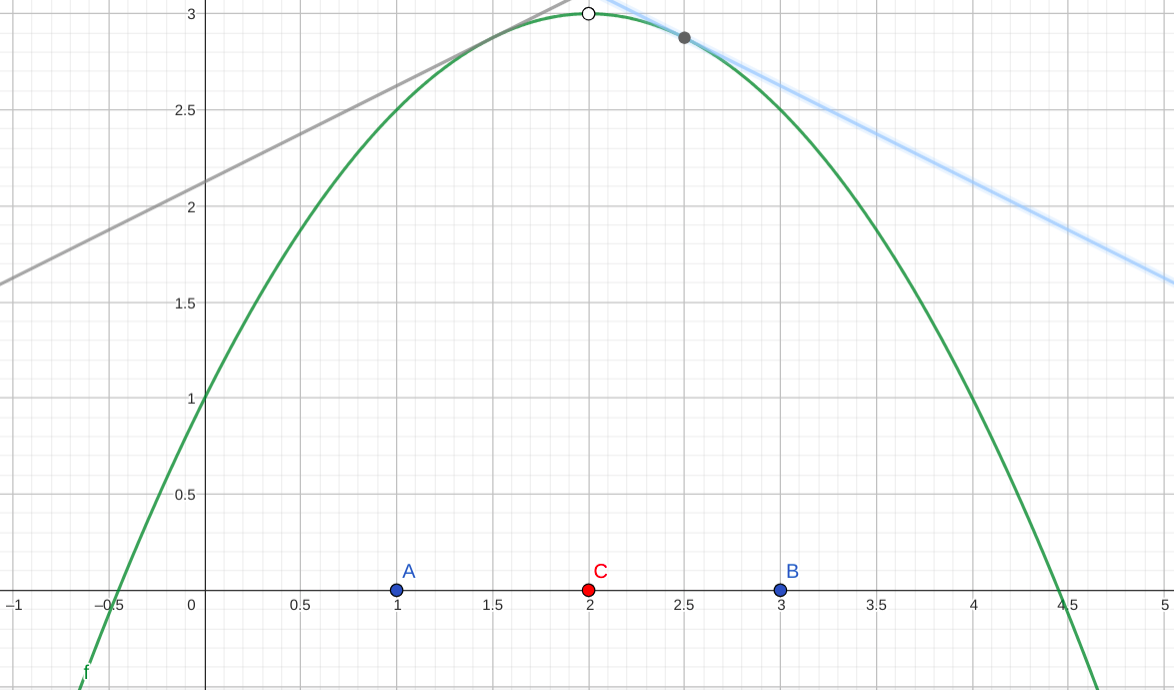
\includegraphics[scale=0.2]{images/noRutinarios1,1.png} \\
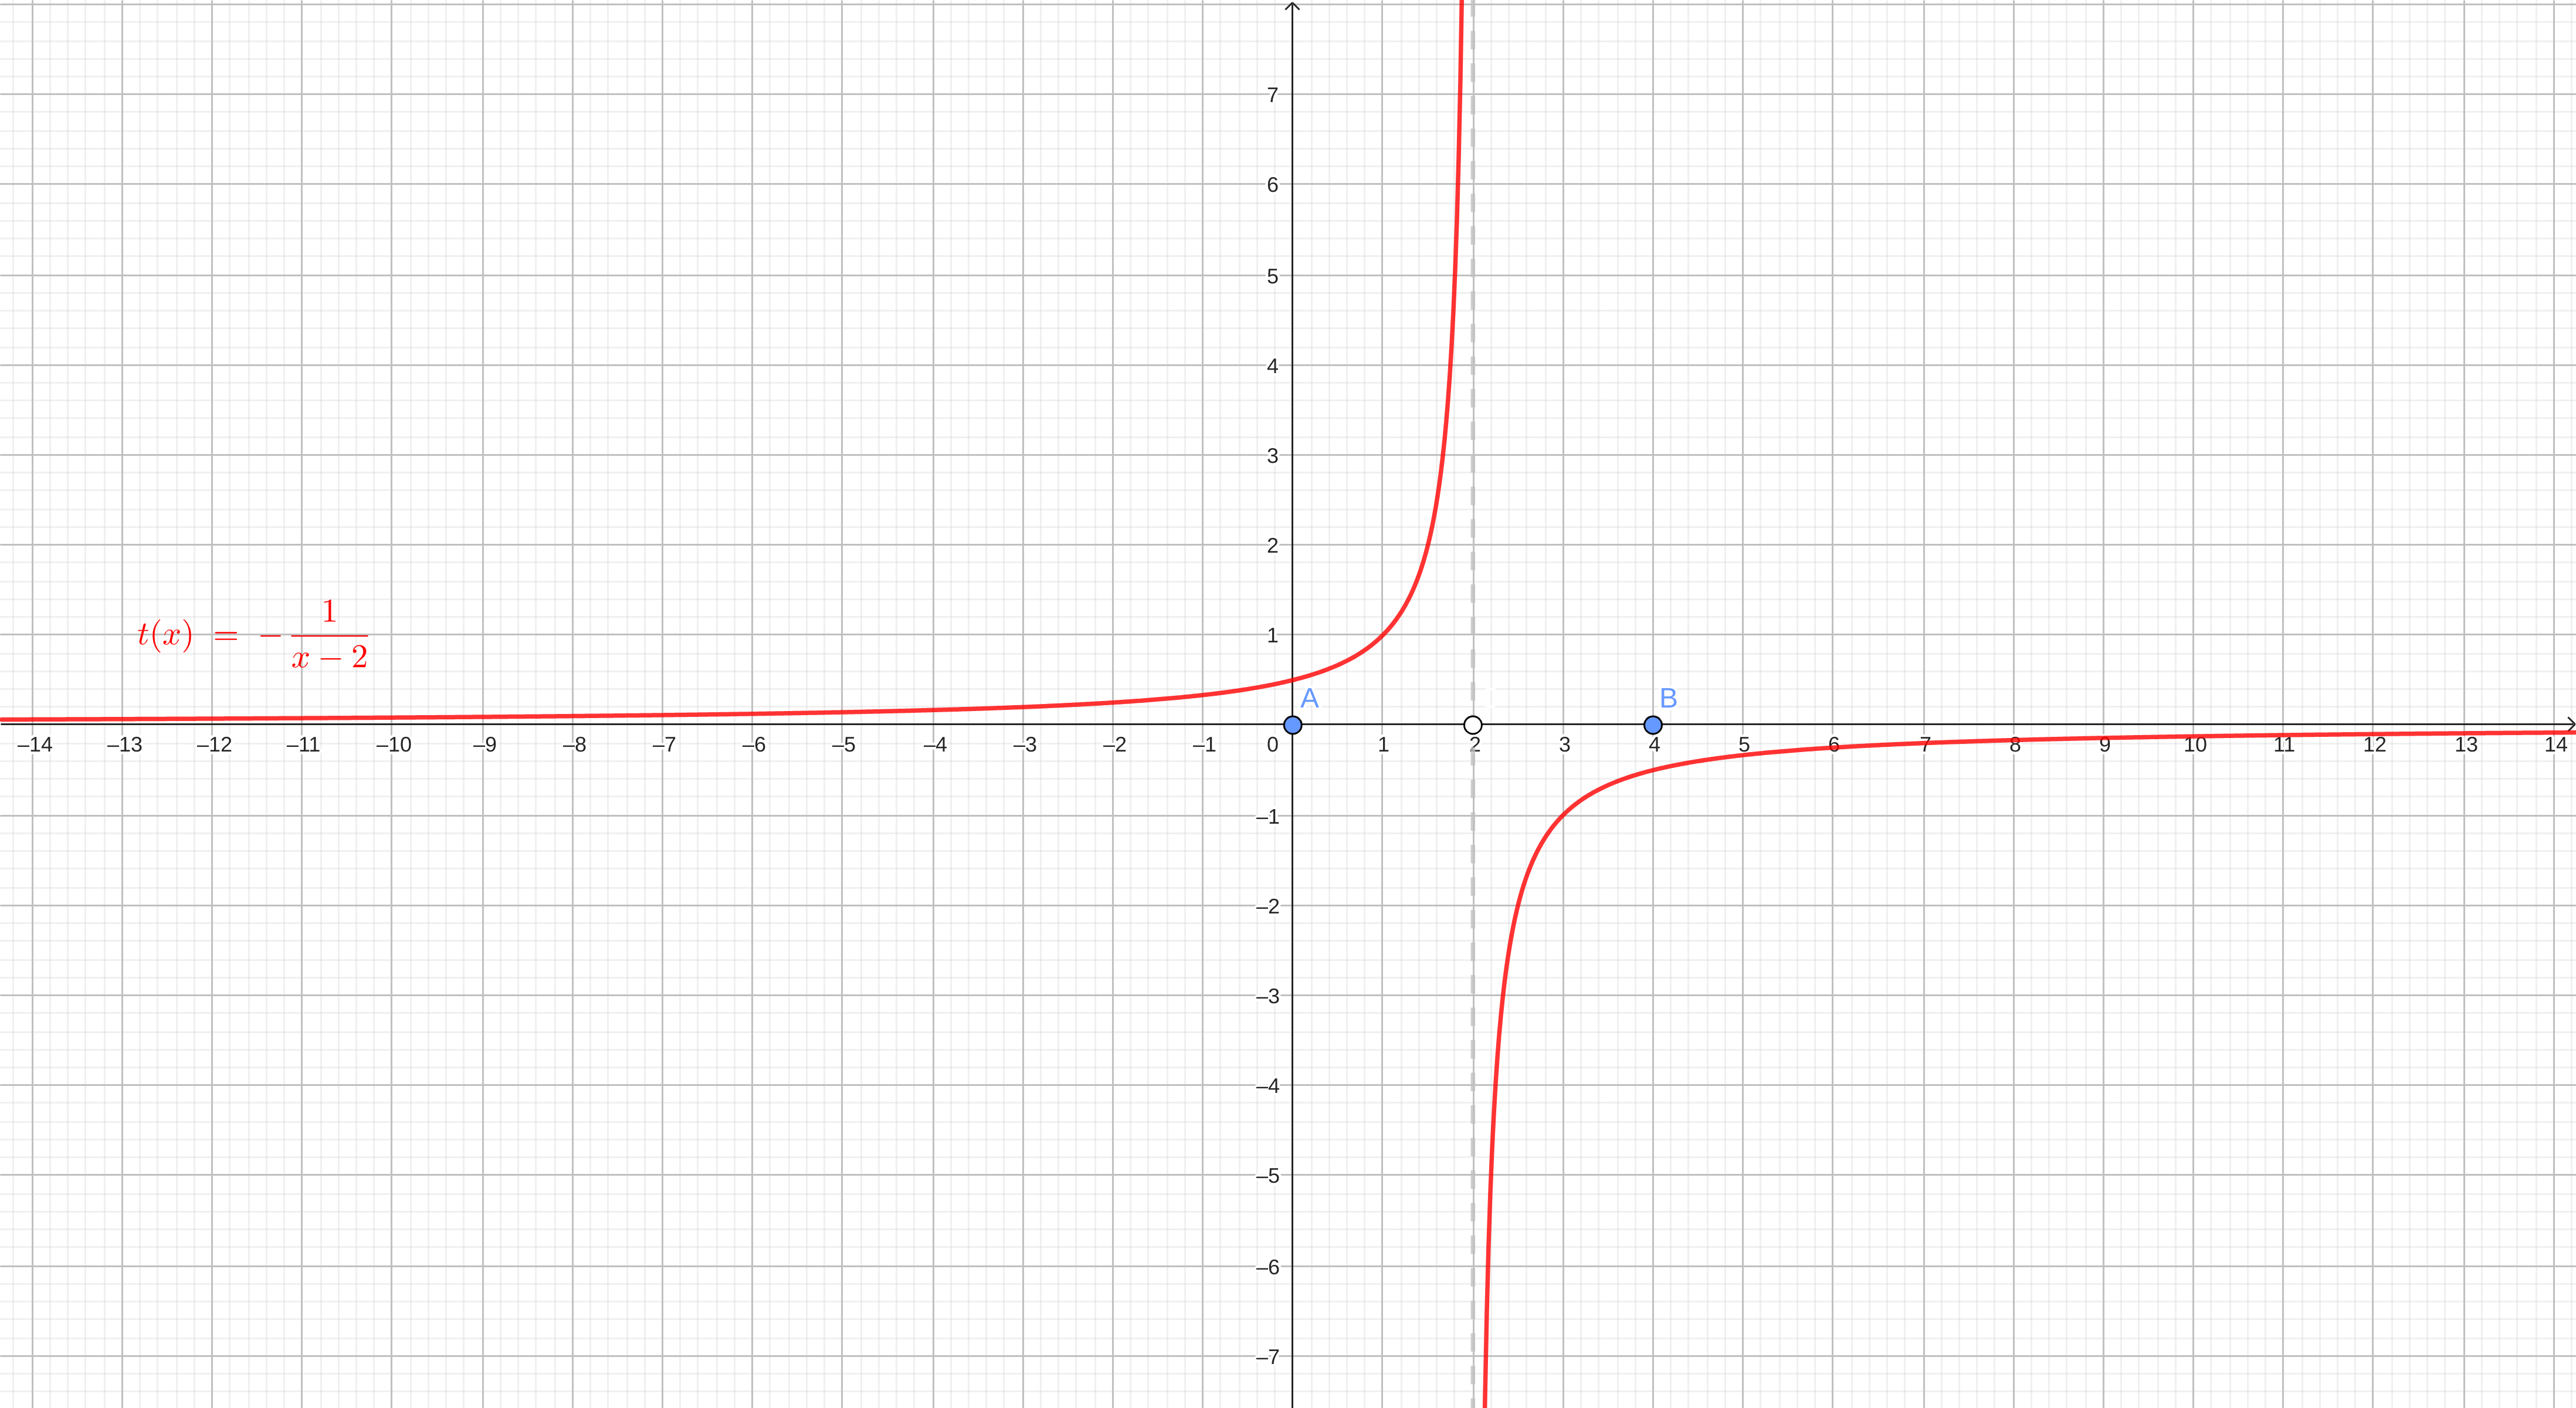
\includegraphics[scale=0.05]{images/noRutinarios1,2.png}